\chapter{Introductory Concepts of Astrophysics}
\label{chap:introductory-concepts-of-astrophysics}
\thispagestyle{empty}

In 2011, Saul Perlmutter, Adam G. Riess, and Brian P. Schmidt received the Nobel Prize in Physics \enquote{for the discovery of the accelerating expansion of the Universe through observations of distant supernovae}. \footnote{\href{https://www.nobelprize.org/prizes/physics/2011/press-release/}{Press release: https://www.nobelprize.org/prizes/physics/2011/press-release/}} \\
Since then, we know that the expansion of the universe is accelerating.
The cause of this accelerated expansion is still unknown, but there are some theoretical models which attempt to explain this phenomenon. \\

\noindent The established model in recent cosmology is the \textbf{$\Lambda$CDM-model}, sometimes referred as the \textit{standard model of cosmology}.
In this model, the cause of the accelerated expansion is due to the so called \textit{cosmological constant} $\Lambda$, which appears as a physical constant in Einstein's field equations of general relativity like the Newtonian gravitational constant $G$. \\

\noindent Another model, published in April 2000 by Gia Dvali, Gregory Gabadadze and Massimo Porrati, -- the \textbf{DGP-model} -- proposes a modification of Einstein's field equations by introducing a fifth dimension to the four-dimensional spacetime, so that gravity behaves equivalently to Newtonian gravity on small distances, but weakens on large scales. \\


\noindent Before going into details about both cosmological models, let me introduce relevant concepts in physics and astronomy from which we can relate measurable physical quantities, like the brightness of stars or their redshift, to more abstract properties of the universe like its scale factor. Based on certain assumptions of a theory, it is possible to develope models that make predictions about properties of the universe, for example, how the expansion and its evolution in time influences the relation of physical quantities.



\section{Distance Measurement in Astronomy}

Essential to astronomical observations and measurements is to determine the distance to objects in space like stars, star clusters, galaxies or even clusters of galaxies. \\
By looking at night into the sky, the only information perceived by our human eye are the brightness and some color in which objects (mostly stars) appear.
How do we determine the distance to those objects?


\subsection{The Parallax Method}

One method to determine the distance to an object is by using the \textit{parallax effect}. \\
For this method, we assume that the observed object is almost stationary relative to earth.
First, we detect the position of the measured object in the sky. After a while (for example, after a half year), the object appears at a slightly different position in the sky, since earth moved on its elliptical orbit which leads to another point of view for the observation.
\begin{figure}[H]
    \centering
    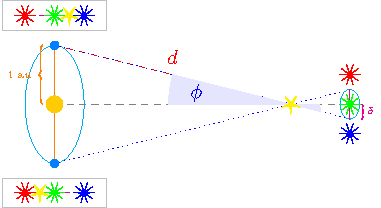
\includegraphics[scale=1.8]{figures/tikz/parallax/parallax.pdf}
    \caption{To determine the distance $d$ between earth and the yellow star, we consider the small change of the position $\delta$ around the green star under which the yellow star appears. The difference $\delta$ relates to the angle $\phi$.}
    \label{fig:parallax}
\end{figure}
\noindent By measuring the appeared difference $\delta$ of the object's position and relating this difference to the angle $\phi$ under which the object changed its position in the sky, we can calculate the distance $d$ by 
\begin{align}
    d = \frac{\SI{1}{\au}}{\sin(\phi)} \approx \frac{\SI{1}{\au}}{\phi},
\end{align}
where $\SI{1}{\au} \approx \SI{149.6e+9}{\meter}$ (``astronomical unit''\footnote{Since 2012, the astronomical unit was redefined by the IAU (International Astronomical Union) to be exactly $\SI{1}{au} := \SI{149597870700}{\meter}$, see \textit{Resolution B2} at the XXVIII General Assembly of IAU: \href{https://www.iau.org/static/resolutions/IAU2012\_English.pdf}{https://www.iau.org/static/resolutions/IAU2012\_English.pdf}}) is defined as the average distance $d_{\earth \odot}$ of earth to the sun. \\ 
The small-angle approximation can be considered justified, since the distance to earth nearest star (beyond of our solar system), Proxima-Centauri, is about $d_{\text{P.C.}} \approx \SI{4.2}{\ly}$ and therefore $\phi_{\text{P.C.}} \approx \arcsin \bigl( \frac{\SI{1}{\au}}{\SI{4.2}{\ly}} \bigr) \approx \SI{3.723e-6} \ll 1$.
The larger the distance to the measured object, the smaller the angle is. \\
\noindent Since the parallax method is one of the most important ways to measure the distance far away objects, we define the distance of a \textit{parsec} (``parallax second'') as the distance to an object, under which the parallax is $\phi = \SI{1}{\arcsec} = \frac{1}{3600} \SI{}{\degree}$:
\begin{align}
    \SI{1}{\parsec} := \frac{\SI{1}{\au}}{\sin \bigl( \frac{1}{3600} \SI{}{\degree} \bigr)} \approx \SI{3.26}{\ly} \approx \SI{3.086e16}{\meter}.
\end{align}

\noindent This is the usual unit by which cosmological distances or parameters are expressed, for example the \textit{Hubble constant} $H_{0} \approx \SI{67.66}{\frac{\kilo \meter}{\second} \mega \parsec^{-1}}$\footnote{The value of $H_{0}$ according to the results of the \textit{Planck Collaboration 2018}, \cite[Table 7]{Planck2020} }. \\ 

\noindent We should keep in mind that this method has of course boundaries and is practically useful for the local region of our galaxy, since the larger the distance to an observed object is, the apparent change in position in the sky gets smaller and is almost unnoticable for objects with a distance on cosmological scale ($d \gtrsim \SI{300}{\mega \parsec}$). 

\subsection{The Distance Modulus}

Another method to determine the distance to an object with a certain luminosity $L$ is to measure its radiant flux $F$ at a distance $d$ by
\begin{align}
    F = \frac{L}{4\pi d^2}. \label{eq:radiant-flux} 
\end{align}
In general astronomical observations, it is not the radiant flux of a star that is measured. Rather, we observe \textit{differences} of brightness or magnitude $m$ between two objects. We define a difference in magnitude between two objects $m_{1} - m_{2} =: \Delta m$ so that the radiant flux $F_{2}$ of object 2 is 100 times higher than the radiant flux $F_{1}$ of object 1 when their difference in magnitude is $\Delta m = 5$, so 
\begin{align}
    \frac{F_{2}}{F_{1}} = 100 \Leftrightarrow m_{1} - m_{2} = \Delta m = 5.
\end{align}
This leads us to the relation between the difference of magnitude $\Delta m$ and the relation of the radiant flux of two objects
\begin{align}
    \frac{F_{2}}{F_{1}} = 100^{\frac{m_{1} - m_{2}}{5}} 
\end{align}
and therefore with \eqref{eq:radiant-flux}
\begin{align}
    m_{1} - m_{2} = \frac{5}{2} \log_{10} \biggl( \frac{F_{2}}{F_{1}} \biggr) = \frac{5}{2} \log_{10} \biggl( \frac{L_{2}}{4\pi d_{2}^2} \frac{4\pi d_{1}^2}{L_{1}} \biggr) = \frac{5}{2} \log_{10} \biggl( \frac{L_{2}}{L_{1}} \biggr) + 5 \log_{10} \biggl( \frac{d_{1}}{d_{2}} \biggr). \label{eq:rel-magnitude-distance-relation} 
\end{align}
So, to calculate the distance to one of both objects, for example object 2, would require us to know their \textit{relative} magnitudes $m_{1}$ and $m_{2}$, their luminosities $L_{1}$ and $L_{2}$ and the distance $d_{1}$ to object 1. \\
To eliminate the need of knowing five quantities, we can define an \textit{absolute} magnitude $M$ as the magnitude an object would have at a distance of $d = \SI{10}{\parsec}$. If we consider only one object, we therefore can calculate the distance to this object by
\begin{align}
    m - M = \frac{5}{2} \underbrace{\log_{10} \biggl( \frac{L}{L} \biggr)}_{ = 0} + 5 \log_{10} \biggl( \frac{d}{\SI{10}{\parsec}} \biggr) = 5 \log_{10} \biggl(\frac{d}{\SI{10}{\parsec}}\biggr). \label{eq:distance-modulus} 
\end{align}
We call the difference between the relative magnitude $m$ and the absolute magnitude $M$ of one object its \textit{distance modulus}. \\
The benefit of the distance modulus is that we only have to know two quantities, $m$ and $M$, to calculate the distance to an object. \\
Unfortunately, we cannot measure the absolute magnitude $M$ of an object that easily (since we can not fly to far away stars and measure the observed magnitude or radiant flux at a distance of $\SI{10}{\parsec}$ to them), which is why we rely on Equation \eqref{eq:rel-magnitude-distance-relation}.
However, we could reduce the amount of unknown variables by calibrating the relation \eqref{eq:rel-magnitude-distance-relation} with an object which luminosity and distance is known. \\

\noindent One could choose to calibrate Equation \eqref{eq:rel-magnitude-distance-relation} by measuring the properties of the nearest star to earth -- our sun. Given the magnitude $m_{\odot}$, the luminosity $L_{\odot}$ and the distance to sun $d_{\earth \odot} = \SI{1}{au}$, we obtain 
\begin{align}
    m = m_{\odot} - \frac{5}{2} \log_{10} \biggl(\frac{L}{L_{\odot}}\biggr) + 5 \log_{10} \biggl(\frac{d}{\SI{1}{au}}\biggr). 
\end{align}

\noindent By this calibration, we could determine the distance to an observed object, if we knew its luminosity $L$ and measured its relative magnitude $m$. Generally, the luminosity of objects like stars could varying arbitrarily. To obtain a reliable distance measurement, we are looking for objects whose luminosity can be predicted very precisely -- so called \textit{standard candles}. \\



\subsection{Possible Candidates for Standard Candles} 

Generally, there are two established candidates for standard candles in astronomy. Since we deal in this thesis with data of type Ia supernovae, the focus lies on the second paragraph of this subsection. For the sake of completeness, however, the cepheids as possible standard candles should not be unmentioned -- also to emphasize why we rely on supernovae of type Ia to determinine cosmological distances.

\subsubsection{Cepheids}

There are several types and classes of cepheids, but they all have in common that those stars obey a certain, periodic relation of luminosity and time. \\

\noindent Without going into details\footnote{For further information and more detailed explanation how stellar pulsation and its underlying $\kappa$-mechanism can be calculated, I recommend chapter 14 ``\textit{Stellar Pulsation}'' in \cite{BradleyCarroll2007}} the periodicity of luminosity is caused by fluctuations of temperature dependent opacity in the stars photosphere due to transitions between single- and dual-ionized Helium inside the star. 

\noindent It is important to identify cepheids of the same type -- cepheids that share the same physical properties, like their metalicity or the same periodicity pattern in their luminosity, to ensure that the same physical process is occuring in all cepheids of a certain type.
\noindent From then on, it is possible to determine the luminosity of all cepheids of the same type by observing one cepheid, measuring its relative magnitude $m$ and its distance $d$ by the parallax method. \\

\begin{figure}[H]
    \centering
    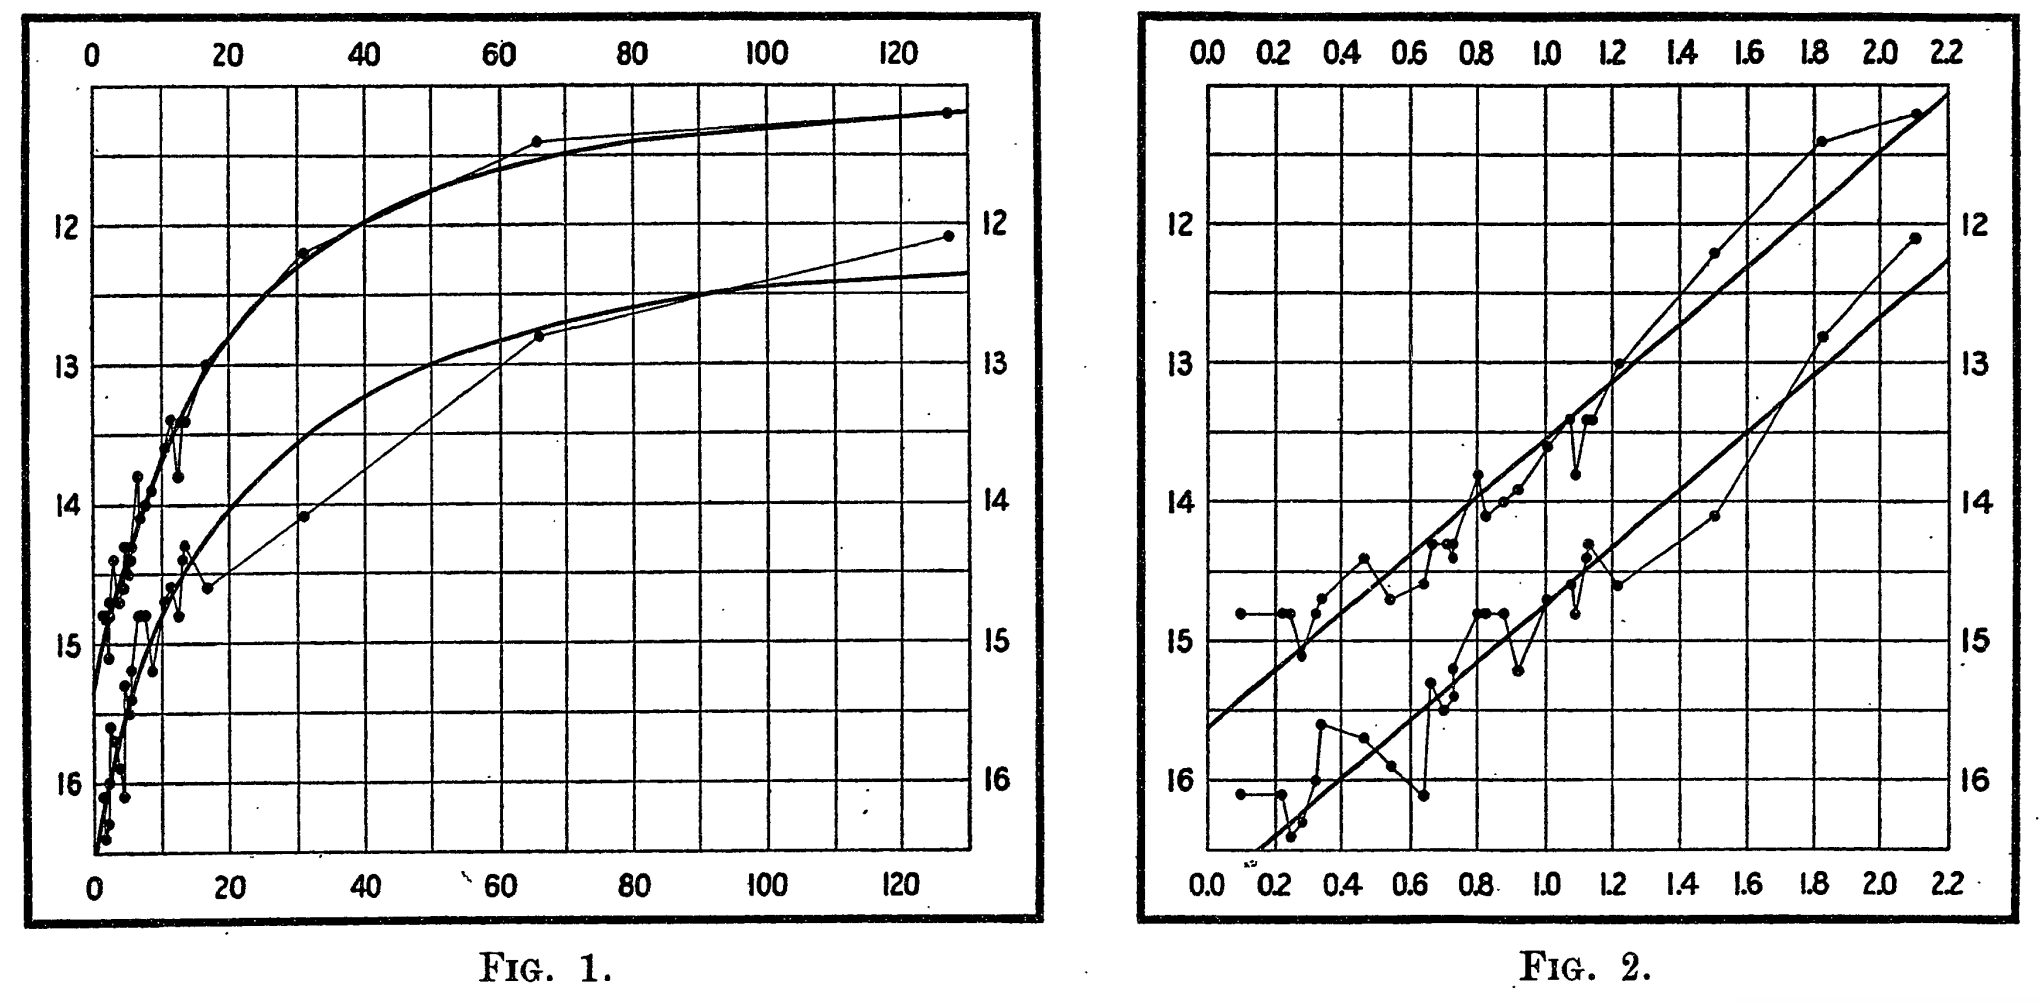
\includegraphics[scale=0.3]{figures/images/leavitt_period-luminosity.png}
    \caption{First observed direct, logarithmic periodicity between time ($x$-axis in days) and magnitude ($y$-axis) of 25 stars in the Small Magellanic Cloud by Henrietta Leavitt, published 1912. Source: \cite{Leavitt1912}.}
\end{figure}


\noindent However, in order to use cepheids for distance determination, they must first be observed and resolved.
Even with our most powerful telescopes that we have today, resolution of cepheids is only possible in our local, galactic neighborhood, for example in the Large Magellanic Cloud or the Andromeda galaxy. Therefore, the boundary to resolute cepheids in other galaxies is currently about $\sim \SI{30}{\mega \parsec}$ (\cite[p.~47]{Bartelmann2019} and \cite[p.~3]{Engelmann2013}). \\
For larger scales, we need much brighter standard candles.



\subsubsection{Supernovae of Type Ia}

In general, supernovae are abrupt bursts of luminosity from massive stars, often accompanied by explosive thermonuclear reactions.
While supernovae of type Ib, Ic and II occur due to an imbalance between the star's gravity, which causes its nucleus to collapse, and radiation emitted by nuclear fusion inside the star, which pushes against its photosphere, supernovae of type Ia are caused by a white dwarf accreting a companion star and therefore increasing in mass. \\
If, due to accreating a companion star, the white dwarf reaches star a mass limit over $\sim 1.4 M_{\odot}$ (where $M_{\odot} \approx \SI{1.98e+30}{\kilogram}$ is the mass of the sun, \cite[p.~48]{Bartelmann2019}), which is called the \textit{Chandrasekhar limit} $M_{\text{Ch}}$, the nucleus of the white dwarf beocmes unstable, since the degeneracy pressure of the electrons (Pauli exclusion principle) cannot resist the gravitational forces any more. \\
Inside the white dwarf's nucleus, a fusion of carbon and oxygen is triggered, which leads to further nuclear processes and an amount of energy release up to $\sim \SI{e+44}{\joule}$ (\cite[p.~295]{Maguire2017}, \cite[p.~321]{Spatschek2017}).
This makes supernovae of type Ia one of the most energetic -- and therefore also luminous -- phenomena known in nature. Supernovae of type Ia are almost as bright as their host galaxy. 
Since they are not only extremly luminous, but the process of star collapse is triggered after crossing a fixed limit of mass (the Chandrasekhar limit), this makes them also very unique and therefore good candidates for standard candles. \\
\noindent We can distinguish between supernovae of type Ia from other supernovae types by observing and analizing their spectrum.

\begin{SCfigure}[][h]
    \begin{minipage}{7cm}
        \caption{Key features in the spectra of different supernovae types are shaded in grey. \\ 
            While supernovae of type II have significant hydrogen lines, supernovae of type Ia and Ib are lacking of hydrogen lines. In type Ia supernovae, the Si II line (at $\sim \SI{6150}{\angstrom}$) is very significant, while it is weak in type Ib supernovae. In type Ib supernovae, the helium lines seems to be very strong.
     Supernovae of type Ic do have non of the mentioned features. \\
Source: \cite[Figure 1]{Quimby2018}}
    \end{minipage}
    \hspace{1cm}
    \begin{minipage}{7cm}
        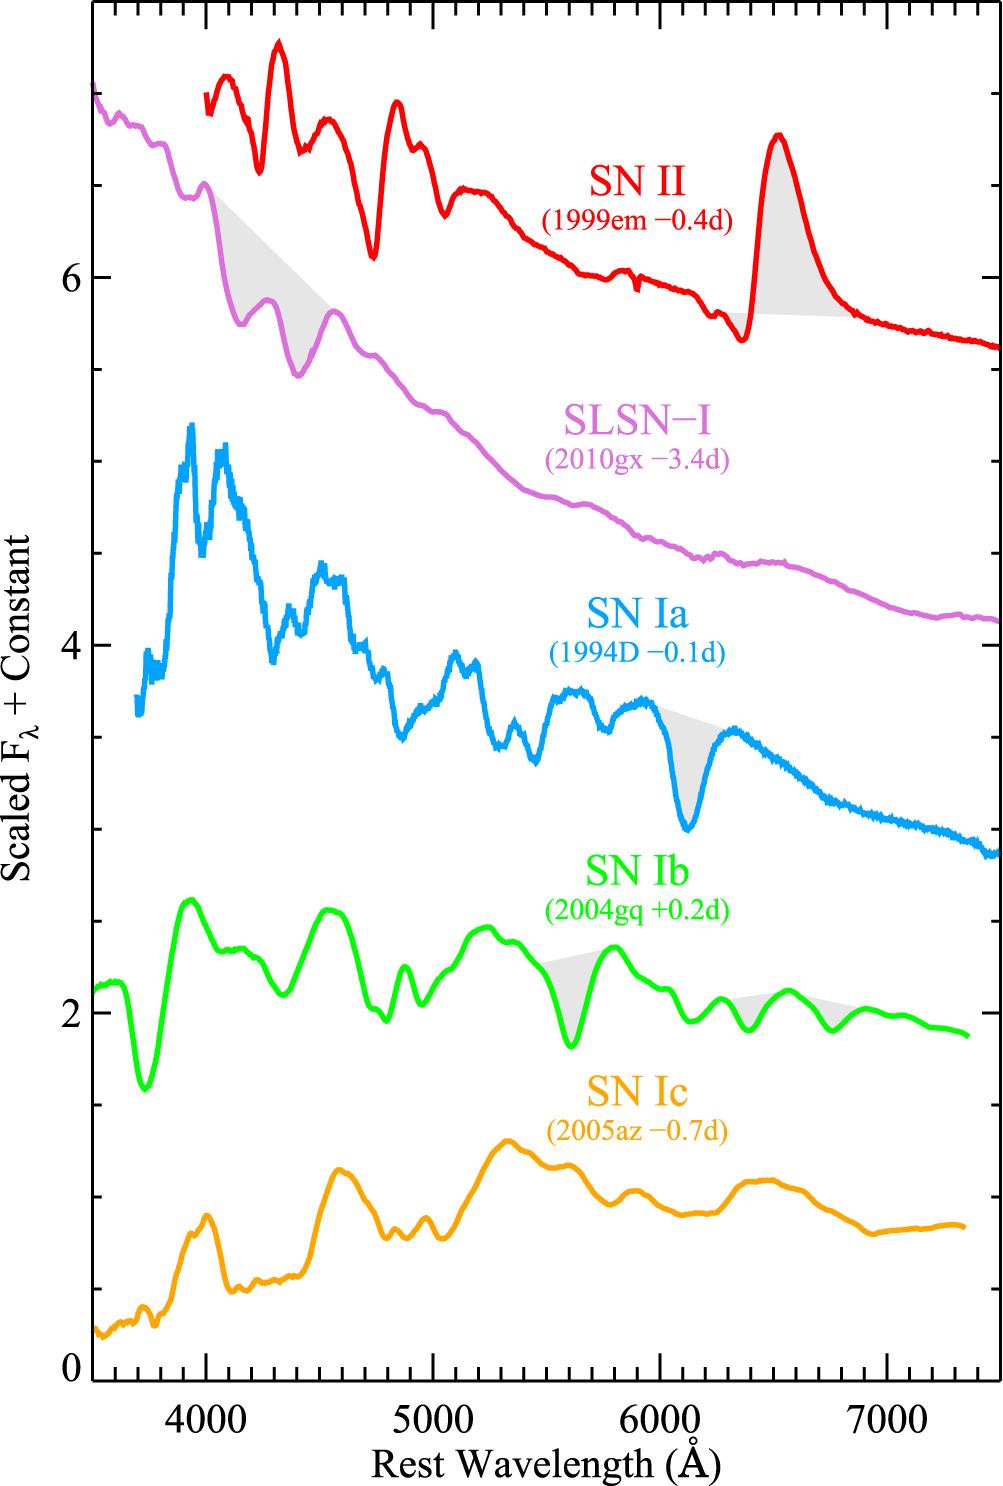
\includegraphics[scale=0.8]{figures/images/supernovae-spectra.jpg}
    \end{minipage}
\end{SCfigure}

\noindent Yet there are small problems that occur here. \\
First, the mechanism which leads to the supernovae explosion is somewhat controversial, since there are two possible scenarios: the ``single-degenerate''-model, in which the companion star is a star of the main sequence or a giant star, and the ``double-degenerate''-model, in which the companion star is also a white dwarf. \\

\noindent In the ``single-degenerate''-model, the accretion must not be too slow, since the hydrogen-rich material of the companion star could be burnt at the same rate as it is accreted, which results in no growth of mass for the white dwarf. On the other hand, the accretion must not be too high, since the accretion might stop due to the companion star's loss of mass at a high rate or being engulfed by the accreted material (\cite[p.~308]{Maguire2017}).

\noindent In the ``double-degenrate''-model, it is assumed that one of both white dwarfs reaches the Chandrasekhar limit if they get too close (\cite[p.~48]{Bartelmann2019}), but there are also other possible scenarios that could occur (see \cite[p.~308/309]{Maguire2017}). \\
\noindent This could lead to slight variations in the luminosity behavior. \\


\noindent Other variations in luminosity behavior could occur due the amount of $^{56}$Ni in the thermonuclear process whose decay influences the peak of the supernovae type Ia light curve (\cite[p.~295]{Maguire2017}). However, those variations can be compensated very well since a relation between the lumninosity's decline and its peak is found so that it is possible to ``normalize'' or ``stretch'' the light curves so they obey a uniform distribution (\cite[p.~4]{Perlmutter2003}, \cite{Phillips1993}).\\
The fact that the light curves of type Ia supernovae are distributed exactly the same way after some ``normalization'' or ``stretching'' shows us that the same physical process underlies all light curves of type Ia supernovae, even if they seem to be stretched, not only due to the relation of luminositys decline and luminosity peak. We will mention later why this property of supernovae type Ia light curves verify the expansion of the universe.

\begin{figure}[H]
    \centering
    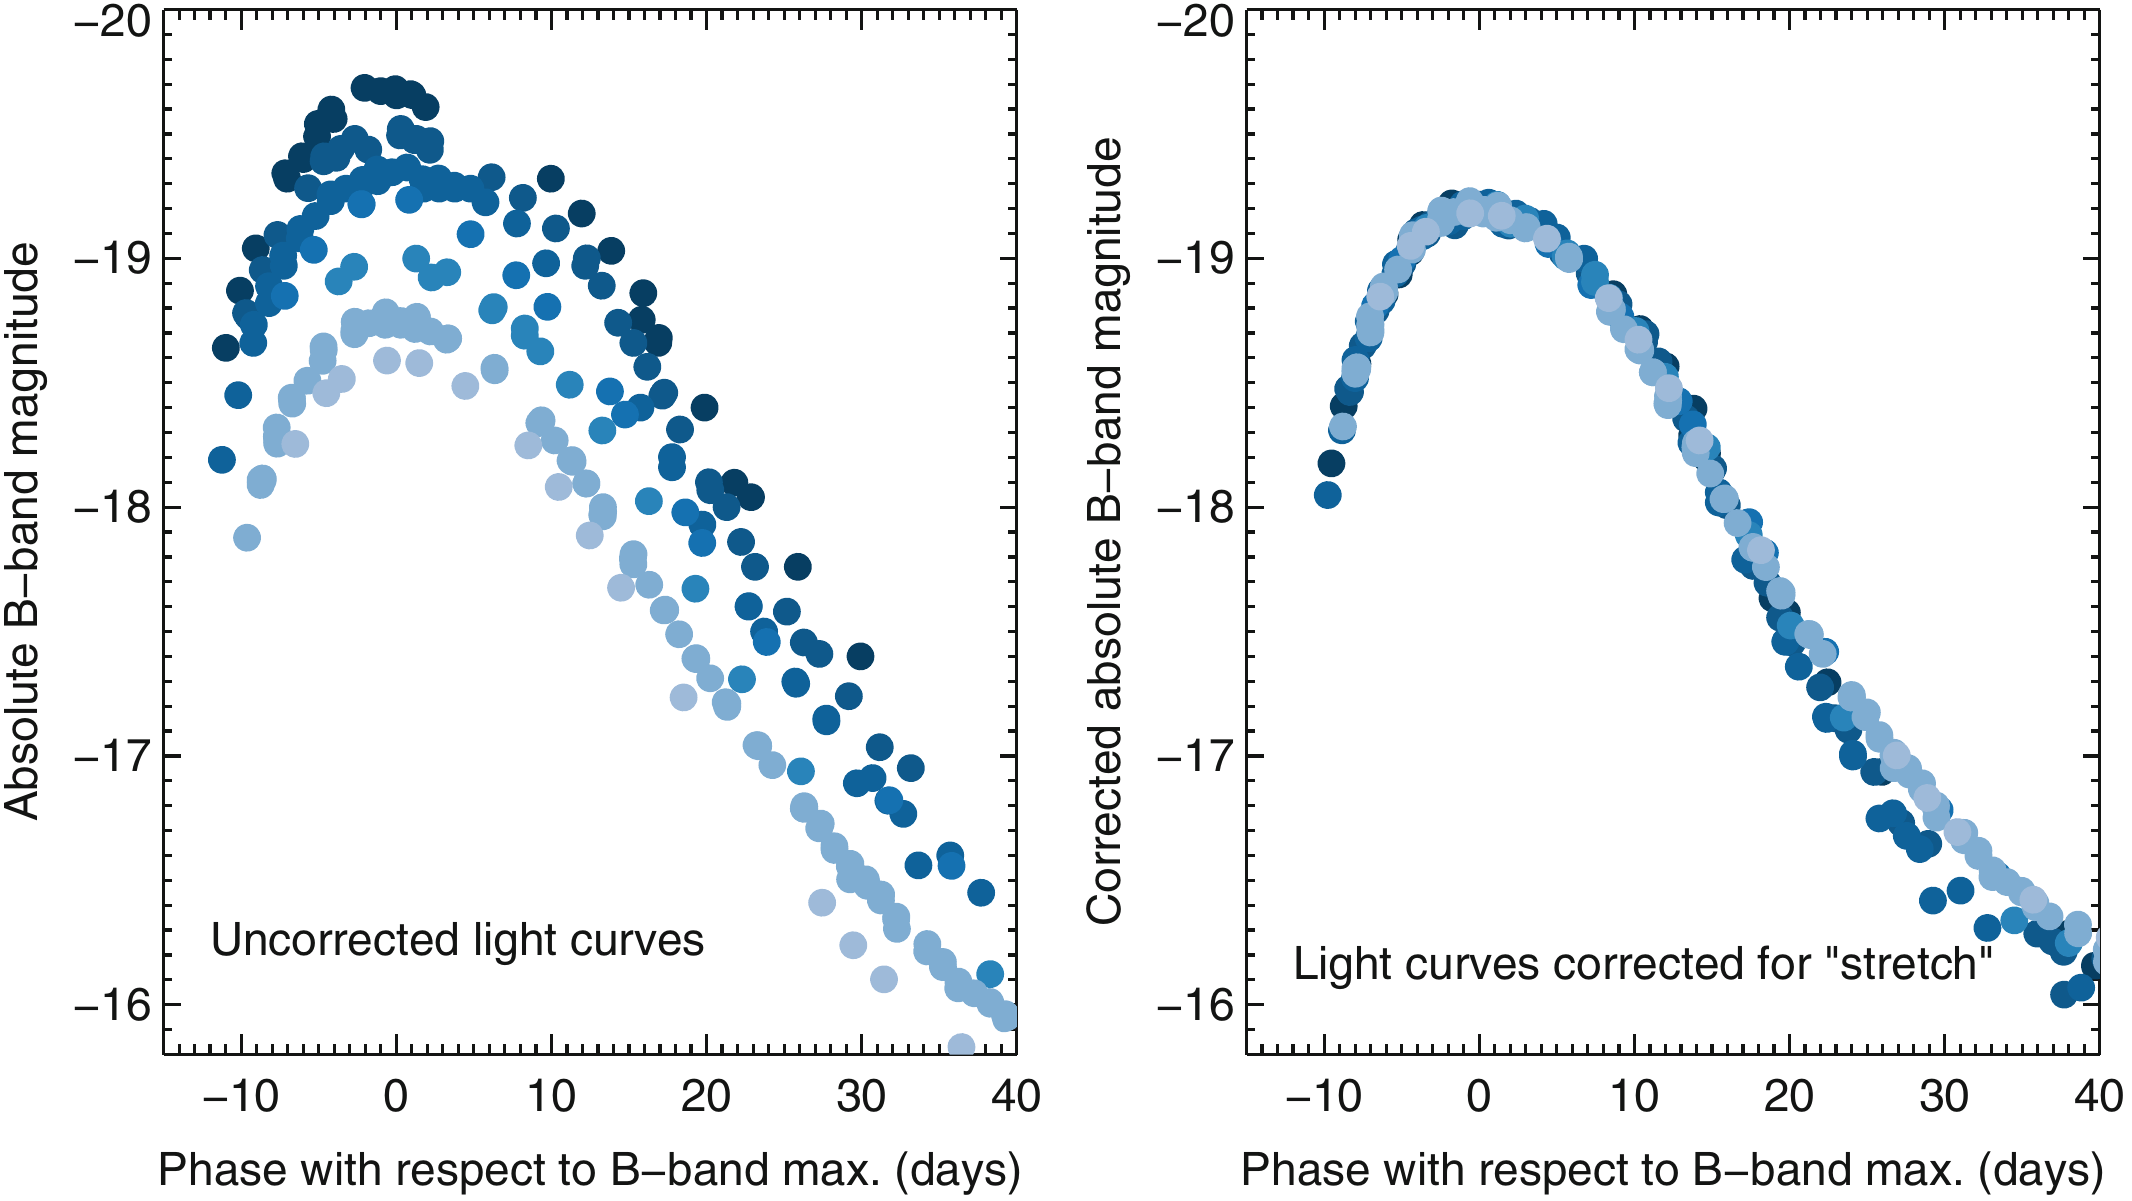
\includegraphics[scale=0.35]{figures/images/supernovae-stretch.png}
    \caption{Uncorrected vs. corrected sample of supernovae type Ia light curves. \\ 
    Source: \cite[p.~298, Figure 2]{Maguire2017}} 
\end{figure}

\noindent Despite the mentioned slight variations in the luminosity spectrum, supernovae of type Ia can be considered as the best candidates for standard candles at the current state of research, not only because their light curves are very homogeneous, but they are also much brighter than cepheids and therefore also visible at large distances, which is essential for cosmological research.


\subsection{Redshift and Hubble's Observation}

The most important tool to determine distances on a cosmological scale is by observing the redshift of extragalactic objects. The redshift is a shift in the observed spectrum of light emmitted by a source with wavelength $\lambda_{\text{e}}$ to an observed wavelength $\lambda_{\text{o}}$ and defined as
\begin{align}
    z := \frac{\lambda_{\text{o}} - \lambda_{\text{e}}}{\lambda_{\text{e}}} = \frac{\lambda_{\text{o}}}{\lambda_{\text{e}}} - 1. \label{eq:redshift}
\end{align}
The term ``red'' in ``redshift'' might be misleading, since $z$ could take also values $<0$ and therefore $\lambda_{\text{o}} < \lambda_{\text{e}}$, which implicates a shift of the light's spectrum to the blue. \\
This term has been established because observations show that the spectrum of most galaxies and extragalactic objects is shifted towards red. \\

\noindent Towards the end of the 1920s, Edwin Hubble observed a certain relation between the measured redshift of the galaxies and extragalactic objects and their distance to us. If one assumes the redshift due to (relativistic) doppler effect,\footnote{Some raised objections against the interpretation that the observed redshift is a result of the doppler effect, but claimed that it is caused by energy loss of the photons traveling through space (``tired light''-hypothesis). We will address later why this hypothesis cannot be hold anymore in the light of tremendous evidence for the expansion model.} one could calculate the galaxies' velocity component towards the direction of observation by
\begin{align}
    z = \gamma \biggl( 1 + \frac{v}{c} \biggr) = \sqrt{\frac{c + v}{c - v}} - 1. \label{eq:relativistic-doppler}
\end{align} 

\noindent An observed shift of the spectrum to the red would imply that the observed object moves away from the observer, and a shift of the spectrum to the blue implies a motion towards the observer. \\
\noindent Edwin Hubble applied a linear relation (see Figure \ref{fig:hubble-law}) between the measured distance $d$ to the observed objects and the calculated velocity $v$ due to the doppler effect
\begin{align}
    v = H_{0} d, \label{eq:hubble-law}
\end{align}
which is known as the \textit{Hubble law}. The proportionality constant $H_{0}$ has the dimension of an inverse time. It is one of the most important parameters in cosmology and its precise determination a challenge of active research (often called ``Hubble tension'', \cite{DiValentino2021}). \\ 

\noindent For small velocities ($v \ll c$), we can approximate \eqref{eq:relativistic-doppler} (first order Taylor series) as $\displaystyle z \approx \frac{v}{c}$, which leads with \eqref{eq:hubble-law} to 
\begin{align}
    d \approx \frac{c}{H_{0}} z. \label{eq:lum-dist-approx} 
\end{align}
We will see later that this relation is actually a first order approximation between the \textit{luminosity distance} $d_{\text{L}}$ and the redshift $z$. \\
The correct relation between the luminosity distance $d_{\text{L}}$ and the redshift $z$ will play an essential role when estimating parameters of cosmological models.

\noindent From Hubble's law follows that the further the distance to a galaxy (or other cosmological object) is, the higher the redshift and therefore, the faster it seems to move apart from us. This observation was one of the milestones in the history of cosmology and was the first indicator that our universe is truly expanding.


\begin{figure}[H]
    \begin{minipage}{8cm}
        \centering 
        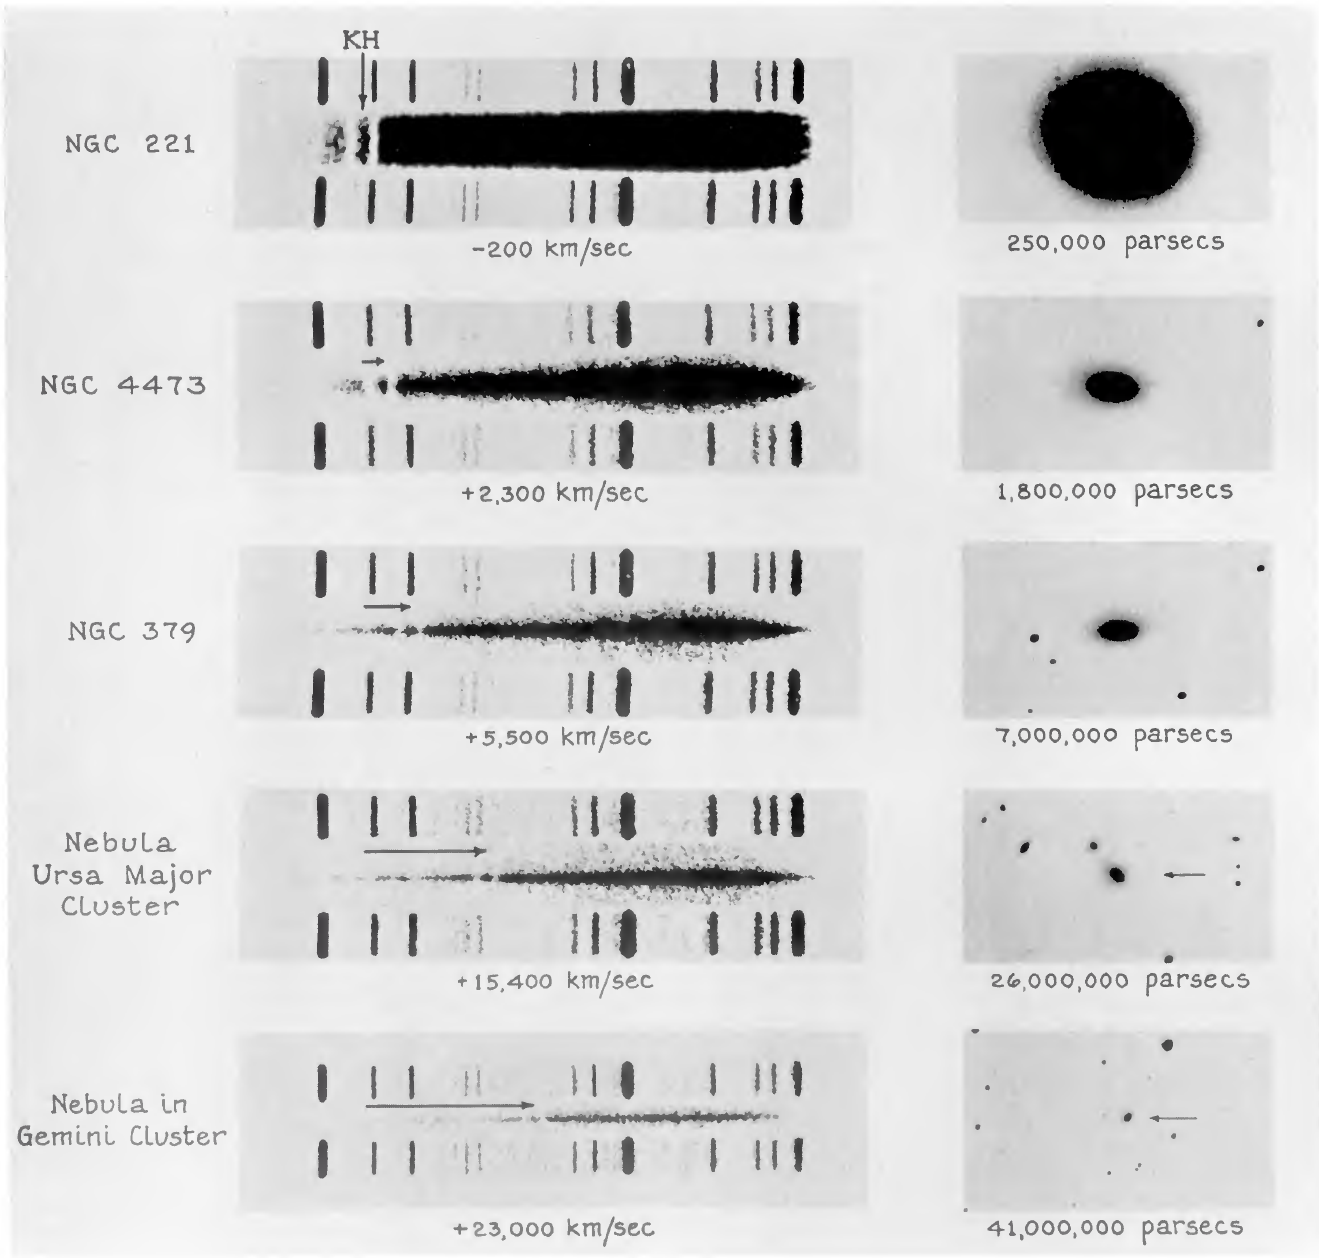
\includegraphics[scale=0.3]{figures/images/humason_redshifts-in-the-spectra-of-extra-galactic-nebulae.png}
        \caption{Observed redshift of H and K lines of calcium, shifted to the red, by Milton L. Humason.  \\ 
        Source: \cite[Figure ``Red-shifts in the Spectra of Extra-galactic Nebulae'']{Humason1936}}
    \end{minipage}
    \hspace{1cm}
    \begin{minipage}{8cm}
        \centering
        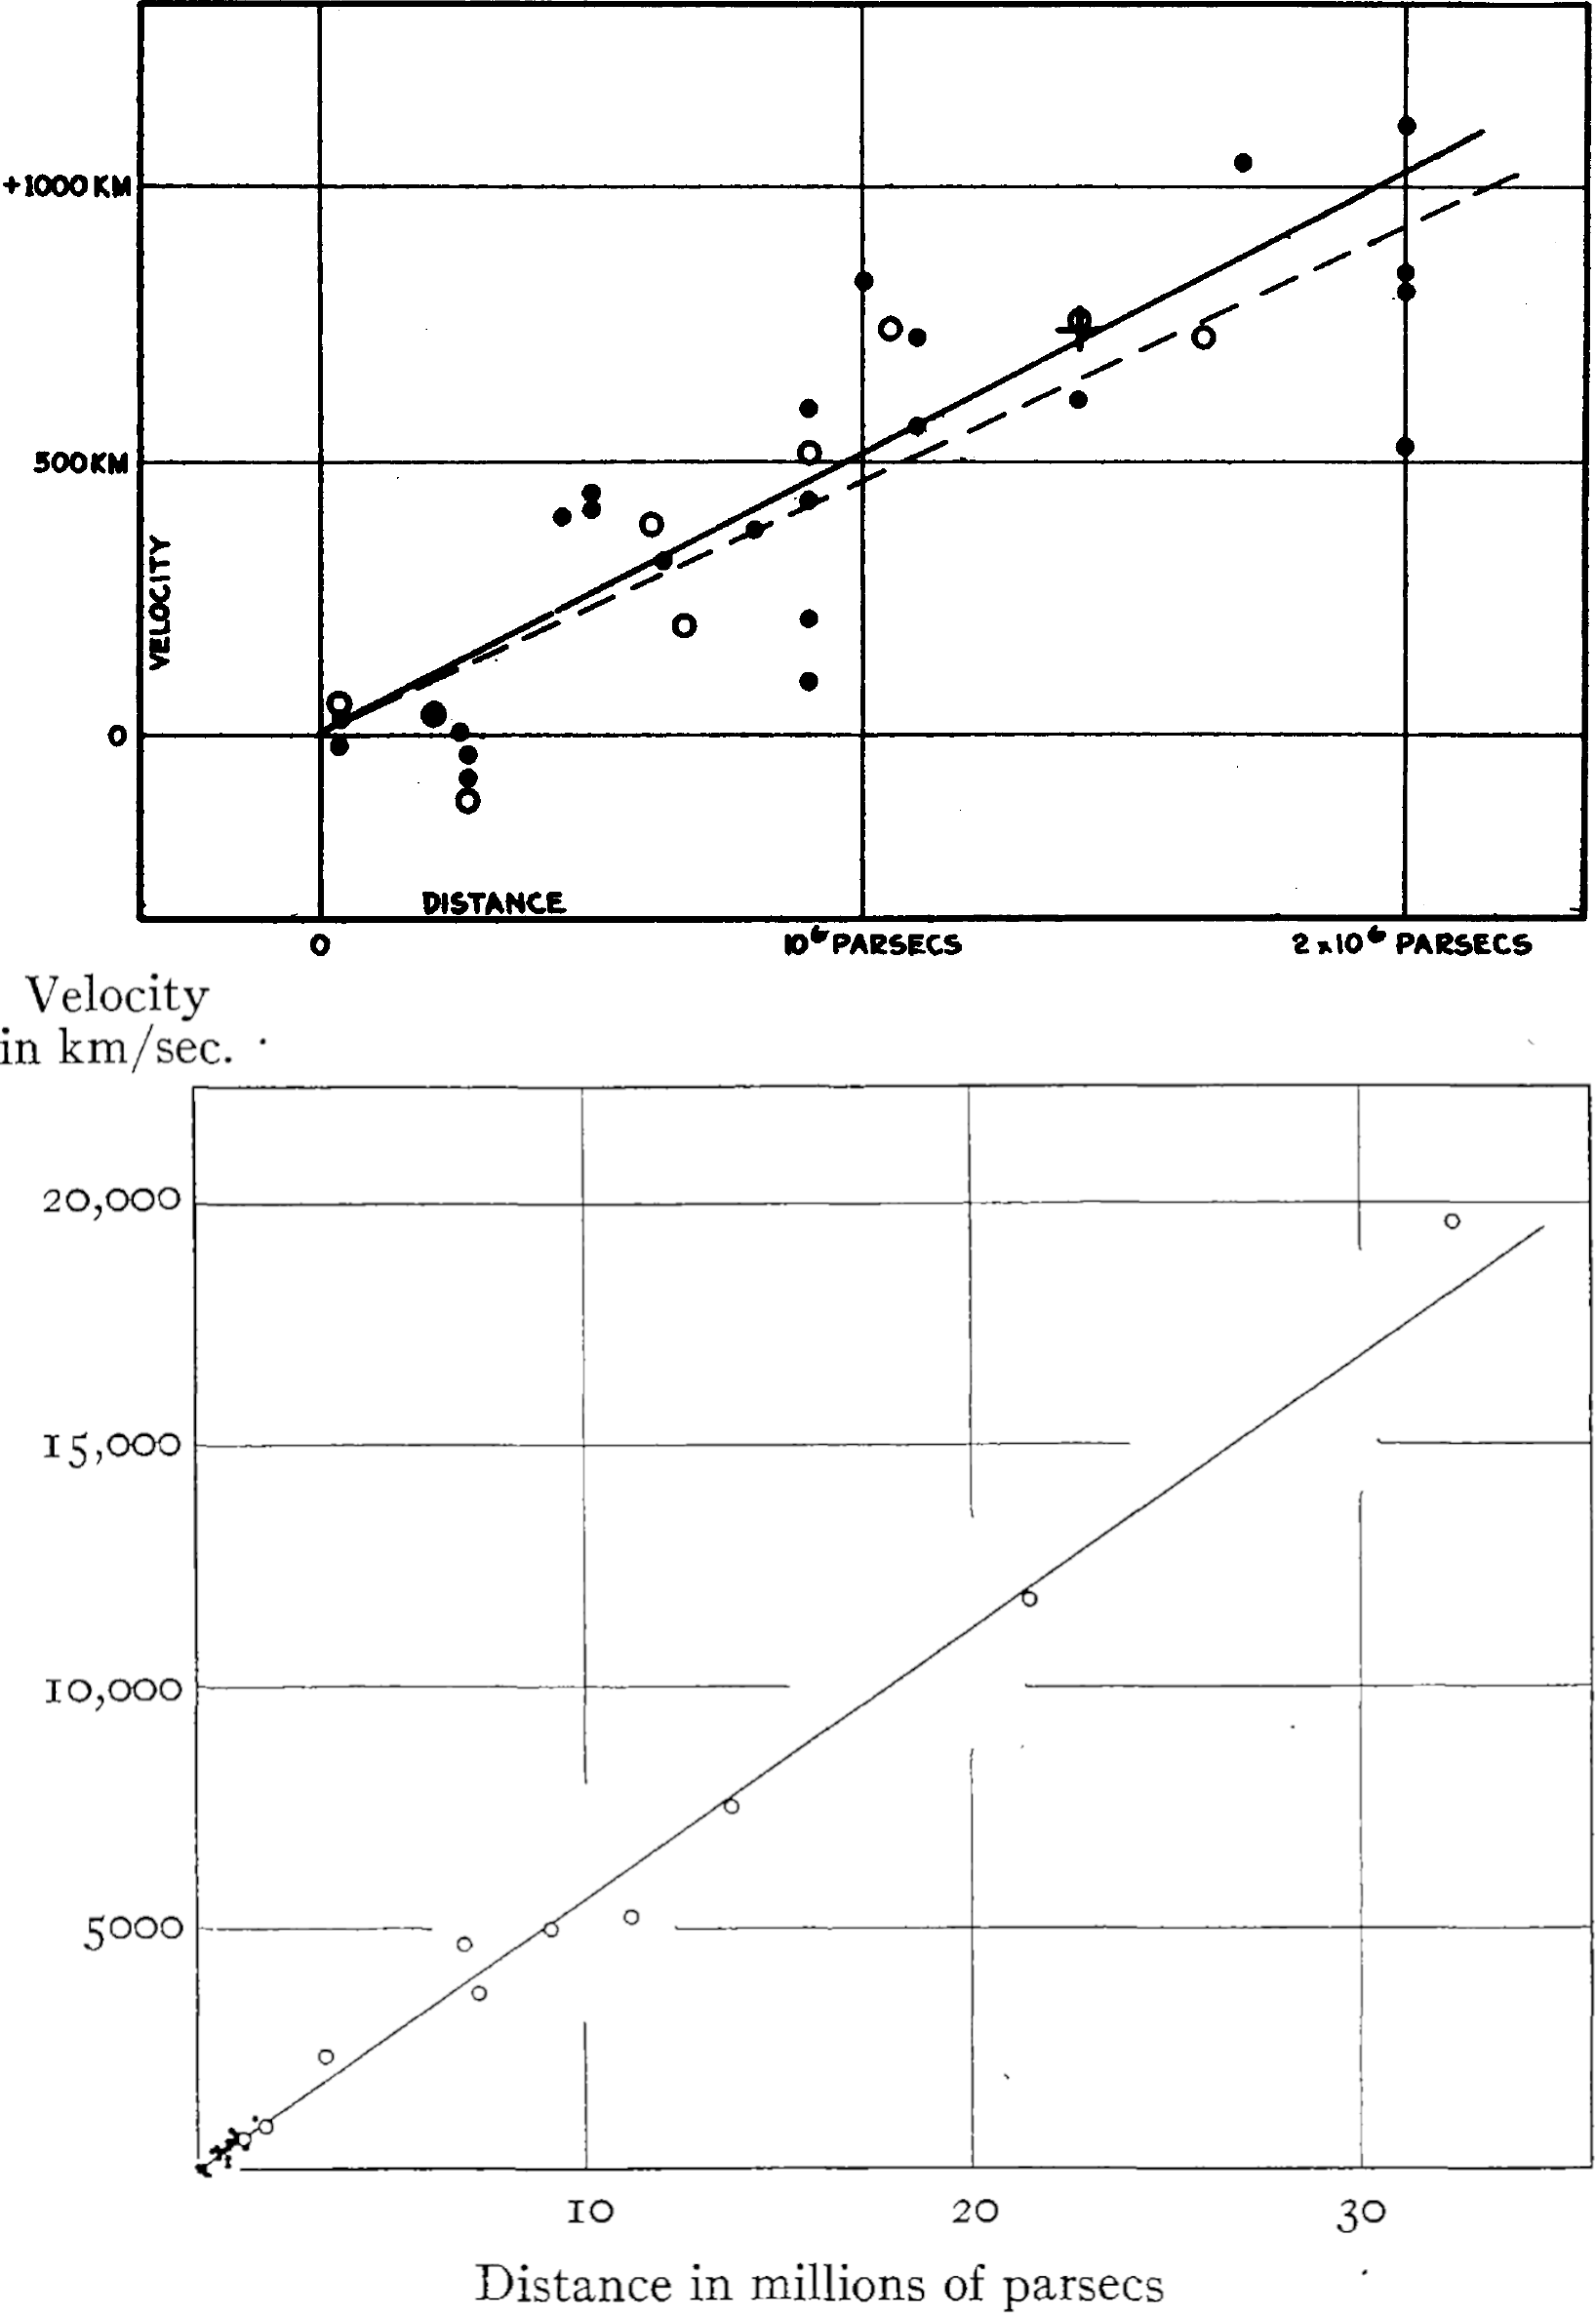
\includegraphics[scale=0.17]{figures/images/hubble_distance-vs-velocity.png}
        \caption{Linear regression between the distance of observed objects and the calculated velocity due to redshift. \\ 
        Source: \cite{Hubble1929} and \cite[Figure 5]{Hubble1931}}
        \label{fig:hubble-law}
    \end{minipage}    
\end{figure}



\section{The Theory of Gravity and Spacetime}
How can one speak about the nature on large scales without mentioning the force that dominates in this regime?
Beginning with Newton's ideas about gravity, the modern formulation about gravity is described in the framework of Einstein's general theory of relativity, in which gravity is, strictly speaking, not anymore a force in the Newtonian sense, but rather a property of the four dimensional spacetime that interacts with matter. \\

\noindent For a deep understanding of general relativity, it is required to have knowledge on the mathematics of differential geometry. \\
\noindent Besides the fact that, as an undergraduate student, I do not (yet) possess this knowledge, this would be beyond the scope of this bachelor thesis. \\
\noindent However, to motivate the basic equations of the $\Lambda$CDM-Model, which are derived from Einstein's field equations under certain assumptions that we are going to formulate in the next chapter, I would like to mention the concept of a \textit{metric} and give brief view on Einstein's field equations.

\subsection{The Metric of Spacetime}
Generally speaking, a metric is a function that takes two points in space and returns a distance. \\
For example, let $\mathbb{E}^2$ be the Euclidean, two dimensional space, then
\begin{align}
    d(\cdot, \cdot) : \mathbb{E}^{2} \times \mathbb{E}^{2} \to \R, (\vb*{p}_{1}, \vb*{p}_{2}) \mapsto d(\vb*{p}_{1}, \vb*{p}_{2}) := \sqrt{(x_{1} - x_{2})^2 + (y_{1} - y_{2})^2} 
\end{align}
would be a function that gives us the distance between two points $\vb*{p}_{1} = (x_{1}, y_{1})^{\intercal}$ and $\vb*{p}_{2} = (x_{2}, y_{2})^{\intercal}$. This distance function $d$ would return the Pythagorean distance in Cartesian coordinates that we are familiar with. \\
Let us define $x := x_{1} - x_{2}$, $y := y_{1} - y_{2}$ and $s := d(\vb*{p}_{1}, \vb*{p}_{2})$ so we could write for the (infinitesimal) distance 
\begin{align}
    \dd{s}^2 = \dd{x}^2 + \dd{y}^2. \label{eq:line-element-cartesian}
\end{align}
Now, let us switch to polar coordinates so that $\vb*{p}_{1} := (r_{1}, \phi_{1})^{\intercal}$ and $\vb*{p}_{2} := (r_{2}, \phi_{2})^{\intercal}$. With the given distance function $d$, we would obtain 
\begin{align}
    d(\vb*{p}_{1}, \vb*{p}_{2}) = \sqrt{(r_{1} - r_{2})^2 + (\phi_{1} - \phi_{2})^2}, 
\end{align}
but this is \textit{not} the same distance as in Cartesian coordinates. The distance that would correspond to the same distance as in Cartesian coordinates (see Equation \eqref{eq:line-element-cartesian}), is
\begin{align}
    \dd{s}^2 = \dd{r}^2 + r^2 \dd{\phi}^2 
\end{align}
with $r:= r_{1} - r_{2}$, $\phi := \phi_{1} - \phi_{2}$. \\
\noindent We have to introduce the \textit{metric tensor} (in most applications of physics a $3 \times 3$- or $4 \times 4$-matrix) that guarantees the invariance of the distance function $d$ under coordinate transformation. \\
We define 
% \begin{align}
%     \begin{pmatrix} 1 && 0 \\ 0 && 1 \end{pmatrix} \overset{\text{cartesian}}{=} g_{ij} \overset{\text{polar}}{=} \begin{pmatrix} 1 && 0 \\ 0 && r \end{pmatrix}, \quad x \overset{\text{cartesian}}{=} x^{1} \overset{\text{polar}}{=} r, \quad y \overset{\text{cartesian}}{=} x^{2} \overset{\text{polar}}{=} \phi, 
% \end{align}
\begin{align}
    g_{ij} := \begin{cases} \begin{pmatrix} 1 && 0 \\ 0 && 1 \end{pmatrix} \quad \text{in cart.} \\  \begin{pmatrix} 1 && 0 \\ 0 && r \end{pmatrix} \quad \text{in polar} \end{cases} x^{1} := \begin{cases} x \quad \text{in cart.} \\ r \quad \text{in polar} \end{cases}  x^{2} := \begin{cases} y \quad \text{in cart.} \\ \phi \quad \text{in polar} \end{cases}
\end{align}
% \begin{align}
%     g_{ij} &\overset{\text{cartestian}}{=} \begin{pmatrix} 1 && 0 \\ 0 && 1 \end{pmatrix} \overset{\text{polar}}{=} \begin{pmatrix} 1 && 0 \\ 0 && r \end{pmatrix}, \quad x^{1} = \begin{cases} x \quad \text{cartestian} \\ r \quad \text{polar}\end{cases},  \quad x^{2} = \begin{cases} y \quad \text{cartesian} \\ \phi \quad \text{polar} \end{cases}
% \end{align}
so that we can express the invariant distance between $\vb*{p}_{1}$ and $\vb*{p}_{2}$ through
\begin{align}
    \dd{s}^2 &= \sum_{i = 1}^{2} \sum_{j = 1}^{2} g_{ij}\dd{x}^{i}\dd{x}^{j} = g_{11} \bigl(\dd{x}^{1}\bigr)^2 + \underbrace{g_{12}}_{= 0} \dd{x}^{1}\dd{x}^{2} + \underbrace{g_{21}}_{= 0} \dd{x}^{2} \dd{x}^{1} + g_{22} \bigl(\dd{x}^{2} \bigr)^2 \\
             &= g_{11} \bigl(\dd{x}^{1}\bigr)^2 + g_{22} \bigl(\dd{x}^{2}\bigr)^2 \overset{\text{cart.}}{=} \dd{x}^{2} + \dd{y}^{2} \overset{\text{polar}}{=} \dd{r}^{2} + r^2 \dd{\phi}^{2}.  
\end{align}

\noindent In the framework of relativity, we express the distance (called ``world line'') between to \textit{events} $\vb*{p}_{1} := (c t_{1}, x_{1}, y_{1}, z_{1})^{\intercal}$ and $\vb*{p}_{2} := (c t_{2}, x_{2}, y_{2}, z_{2})^{\intercal}$ in four dimensional spacetime as
\begin{align}
    \dd{s}^2 = g_{\mu\nu} \dd{x}^{\mu} \dd{x}^{\nu}
\end{align}
with the implicit sum over double occuring indices $\mu, \nu \in \{0,1,2,3\}$. In flat Minkowski-spacetime of special relativity for example, we have 
\begin{align}
    g_{\mu\nu} = \eta_{\mu\nu} := \diag(-1, 1, 1, 1) 
\end{align} 
and therefore for distances in spacetime
\begin{align}
    \dd{s}^2 = \eta_{\mu\nu} \dd{x}^{\mu} \dd{x}^{\nu} = - (c \dd{t})^{2} + \dd{x}^{2} + \dd{y}^{2} + \dd{z}^{2}.    
\end{align}



\subsection{Einstein's Field Equations}

\noindent Similar to the derivation of the Euler--Lagrange equations in classical mechanics (or classical field theory) by formulating an action $S[\vb*{q}(t)]$ (or $S[\phi(x)]$) and find the path $\vb*{q}(t)$ (or field $\phi(x)$) that extremizes the action ($\delta S = 0$), Einstein's field equations can be derived\footnote{For a proper and detailed derivation, see subsection 4.3 ``\textit{Lagrangian Formulation}'' in \cite[p.~159]{SeanCarroll2019}} from the Einstein--Hilbert action given by
\begin{align}
    S_{\text{EH}}[g_{\mu\nu}] = \int \dd[4]{x} \sqrt{-\det(g_{\mu\nu})} \biggl[\frac{c^4}{16\pi G}(R - 2\Lambda) + \mathcal{L}_{\text{M}} \biggr], 
\end{align}
where $\dd[4]{x}$ is the four dimensional spacetime-volume element, $g_{\mu\nu}$ the metric tensor, $c$ the speed of light (in vacuum), $G$ the Newtonian gravitational constant, $R$ the Ricci scalar, $\Lambda$ the cosmological constant, and $\mathcal{L}_{\text{M}}$ the Lagrange density of matter fields. 

\noindent With the action principle, the variation $\delta S[g_{\mu\nu}]$ of the Einstein--Hilbert action with respect to the metric leads to Einstein's field equations
\begin{align}
    R_{\mu\nu} - \frac{1}{2}R g_{\mu\nu} + \Lambda g_{\mu\nu} = \frac{8\pi G}{c^4}T_{\mu \nu}, \label{eq:einstein-field-equations}
\end{align}
where $R_{\mu\nu}$ is the Ricci curvature tensor and $T_{\mu\nu}$ the energy-momentum tensor. \\
\noindent Without getting too much into details about the single components of this equation, we keep in mind that the left hand side of Equation \eqref{eq:einstein-field-equations} describes how spacetime behaves, while the right hand side of Equation \eqref{eq:einstein-field-equations} describes how matter behaves.

\subsubsection{The Cosmological Constant $\Lambda$}

\noindent Originally, Einstein formulated his field equations without the cosmological constant $\Lambda$. Since Einstein believed in a static universe and found that his equations cannot hold for a static universe (it would have collapsed due to the gravity of matter), he introduced the $\Lambda$ term that acts repulsive towards the attraction of gravity, so that a static universe as he proposed would be possible. \\

